\documentclass[10pt]{beamer}
\usetheme{metropolis}

% ── Packages ──
\usepackage{amsmath,amssymb,amsthm}
\usepackage{tikz}
\usetikzlibrary{positioning,arrows.meta,calc}
\usepackage{graphicx}
\usepackage{array}
\usepackage{etoolbox}

% ── Theorem environments ──
\theoremstyle{definition}
\newtheorem{defi}{Definition}[section]
\newtheorem{prop}{Proposition}[section]
\newtheorem{thm}{Theorem}[section]

% Custom theorem styles with colors
\setbeamercolor{block title}{bg=red!75!black,fg=white}
\setbeamercolor{block body}{bg=yellow!10!white}

\AtBeginEnvironment{prop}{%
  \setbeamercolor{block title}{bg=yellow!75!black,fg=black}%
  \setbeamercolor{block body}{bg=yellow!10!white}%
}
\AtEndEnvironment{prop}{%
  \setbeamercolor{block title}{bg=red!75!black,fg=white}%
}

\AtBeginEnvironment{thm}{%
  \setbeamercolor{block title}{bg=yellow!75!black,fg=black}%
  \setbeamercolor{block body}{bg=yellow!10!white}%
}
\AtEndEnvironment{thm}{%
  \setbeamercolor{block title}{bg=red!75!black,fg=white}%
}

% ── Highlighting ──
\newcommand{\x}[1]{\alert{\textbf{#1}}}
\newcommand{\rd}[1]{{\color{red!70!black}#1}}
\newcommand{\bl}[1]{{\color{blue!70!black}#1}}
\newcommand{\gn}[1]{{\color{green!60!black}#1}}
\newcommand{\tl}[1]{{\color{teal!70!black}#1}}
\newcommand{\orthoplus}{\mathbin{\overset{\perp_H}{\oplus}}}

\title{Lecture 19: Normal Matrices}
\subtitle{Hermitian Geometry and Spectral Projections}
\date{}
\titlegraphic{}

\begin{document}
\begin{frame}[plain,shrink=10]
\titlepage
\end{frame}


\begin{frame}{Today's Question}

From previous lectures, spectral decomposition tries to split a matrix into pieces:

$$
A=\lambda_1P_1+\lambda_2P_2+\cdots+\lambda_kP_k.
$$

\vfill

Then every vector splits into eigenspace components:

$$
\mathbf{v}=P_1\mathbf{v}+P_2\mathbf{v}+\cdots+P_k\mathbf{v}.
$$

\vfill\pause

\begin{center}
{\Large \x{Are these pieces perpendicular?}}

\vspace{0.4cm}

{\Large Or are they only oblique algebraic pieces?}
\end{center}

\end{frame}


\begin{frame}{Why Study Normal Matrices?}

Diagonalizable matrices already give spectral decomposition.

\vfill

But diagonalization alone does \x{not} promise geometry:

$$
\mathbb{C}^n=E_{\lambda_1}\oplus\cdots\oplus E_{\lambda_k}
\qquad\text{may be oblique.}
$$

\vfill\pause

Normal matrices are the matrices where spectral decomposition becomes \x{orthogonal geometry}:

$$
\boxed{
\mathbb{C}^n
=E_{\lambda_1}\orthoplus E_{\lambda_2}\orthoplus\cdots\orthoplus E_{\lambda_k}.
}
$$

\vfill

\x{This is why normal matrices matter.}

\end{frame}


\begin{frame}{Two Pictures to Keep in Mind}

\begin{columns}[T,onlytextwidth]
\begin{column}{0.48\textwidth}
\begin{center}
\textbf{Oblique eigenspaces}

\vspace{2mm}
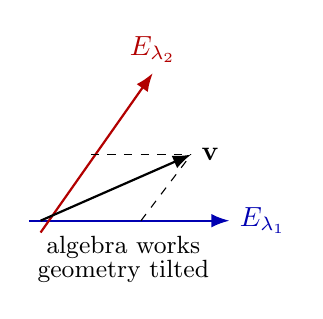
\begin{tikzpicture}[scale=0.75,>=Latex]
  \draw[->,thick,blue!70!black] (-0.2,0) -- (3.2,0) node[right] {$E_{\lambda_1}$};
  \draw[->,thick,red!70!black] (0,-0.2) -- (1.9,2.5) node[above] {$E_{\lambda_2}$};
  \draw[dashed] (1.7,0) -- (2.55,1.12);
  \draw[dashed] (0.85,1.12) -- (2.55,1.12);
  \draw[->,thick] (0,0) -- (2.55,1.12) node[right] {$\mathbf v$};
  \node at (1.4,-0.45) {\small algebra works};
  \node at (1.4,-0.85) {\small geometry tilted};
\end{tikzpicture}
\end{center}
\end{column}
\begin{column}{0.48\textwidth}
\begin{center}
\textbf{Orthogonal eigenspaces}

\vspace{2mm}
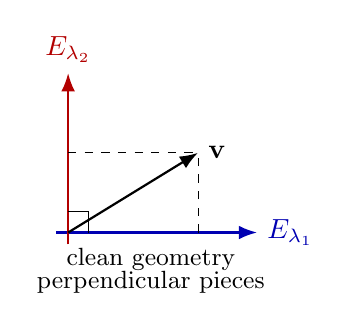
\begin{tikzpicture}[scale=0.75,>=Latex]
  \draw[->,thick,blue!70!black] (-0.2,0) -- (3.2,0) node[right] {$E_{\lambda_1}$};
  \draw[->,thick,red!70!black] (0,-0.2) -- (0,2.7) node[above] {$E_{\lambda_2}$};
  \draw (0.35,0) -- (0.35,0.35) -- (0,0.35);
  \draw[dashed] (2.2,0) -- (2.2,1.35);
  \draw[dashed] (0,1.35) -- (2.2,1.35);
  \draw[->,thick] (0,0) -- (2.2,1.35) node[right] {$\mathbf v$};
  \node at (1.4,-0.45) {\small clean geometry};
  \node at (1.4,-0.85) {\small perpendicular pieces};
\end{tikzpicture}
\end{center}
\end{column}
\end{columns}

\vfill

\begin{center}
\x{Normal matrices answer: when does the right picture happen?}
\end{center}

\end{frame}


\begin{frame}{The Surprising Theorem}

\begin{block}{Main Theorem We Will Prove}
For a complex matrix $A$,
$$
A\text{ normal}
\quad\Longleftrightarrow\quad
\text{all spectral projections }P_i\text{ satisfy }P_i^H=P_i.
$$
\end{block}

\vfill\pause

Equivalently:

$$
A\text{ normal}
\quad\Longleftrightarrow\quad
\text{eigenspaces of }A\text{ are mutually Hermitian-orthogonal.}
$$

\vfill\pause

\x{Not just diagonalizable:} diagonalizable with orthogonal spectral pieces.

\end{frame}


\begin{frame}{How This Connects to Matrix Exponentials}

Lecture 18 gave the spectral formula:

$$
e^{As}=e^{\lambda_1s}P_1+\cdots+e^{\lambda_ks}P_k.
$$

\vfill\pause

If the projections are oblique, the algebra works but the geometry is distorted.

\vfill

If $A$ is normal, then each $P_i$ is an orthogonal projection:

$$
P_i^H=P_i.
$$

\vfill

\x{Meaning:} the system evolves along perpendicular eigenspace directions.

\end{frame}

% ┌─────────────────────────────────────────────────────────────────────┐
% │ SECTION 1: COMPLEX LENGTH FORCES HERMITIAN GEOMETRY                │
% │                                                                    │
% │ ADR: Begin with the failure of v^T v over C. The audience already  │
% │ knows complex numbers from L17 and matrix exponential from L18;     │
% │ this section grounds the new H notation before any normality.       │
% └─────────────────────────────────────────────────────────────────────┘
\section{Complex Length}

\begin{frame}{Why Are We in the Complex World?}

Our spectral method needs roots of the characteristic polynomial:

$$
\det(tI-A)=0.
$$

\vfill\pause

Over $\mathbb{R}$, roots can disappear:

$$
t^2+1=0
\qquad\text{has no real root.}
$$

\vfill

Over $\mathbb{C}$, every polynomial factors into linear factors.

\vfill\pause

\x{So the spectral story naturally lives over $\mathbb{C}$.}

\end{frame}


\begin{frame}{But Complex Geometry Needs Repair}

We want to measure:

\vfill

\begin{itemize}
\item \x{length}: how big is a vector?
\item \x{angle}: when are two vectors perpendicular?
\end{itemize}

\vfill\pause

Over $\mathbb{R}$, we use

$$
\mathbf v^T\mathbf w.
$$

\vfill

Over $\mathbb{C}$, this formula breaks length.

\vfill\pause

\x{Hermitian geometry} is the repaired geometry of complex vector spaces.

\end{frame}


\begin{frame}{The Old Length Formula}

Over real numbers, length comes from

$$
\|\mathbf{v}\|^2=\mathbf{v}^T\mathbf{v}.
$$

\vfill

For
$$
\mathbf{v}=\begin{pmatrix}x_1\\x_2\\ \vdots \\x_n\end{pmatrix}\in\mathbb{R}^n,
$$
we get
$$
\mathbf{v}^T\mathbf{v}
=x_1^2+x_2^2+\cdots+x_n^2.
$$

\vfill

\x{Key:} a nonzero real vector has positive length squared.

\end{frame}


\begin{frame}{What Goes Wrong over $\mathbb{C}$?}

Try the same formula on a complex vector:

$$
\mathbf{v}=\begin{pmatrix}1\\ i\end{pmatrix}.
$$

\vfill\pause

Naive length squared:

$$
\mathbf{v}^T\mathbf{v}
=\begin{pmatrix}1&i\end{pmatrix}
\begin{pmatrix}1\\ i\end{pmatrix}
=1+i^2.
$$

\vfill\pause

But $i^2=-1$, so

$$
\mathbf{v}^T\mathbf{v}=1-1=0.
$$

\vfill

\x{Problem:} a nonzero vector has zero length.

\end{frame}


\begin{frame}[shrink=5]{The Missing Move}

The problem is this multiplication:

$$
\bl{i}\cdot \bl{i}=i^2=-1.
$$

\vfill

For length, we want a positive number:

$$
|i|^2=1.
$$

\vfill\pause

So before taking the dot product, we must mirror the complex number:

$$
\bl{i}\quad\longmapsto\quad \rd{-i}.
$$

\vfill\pause

Then

$$
\rd{(-i)}\cdot \bl{i}=1.
$$

\vfill

\x{Key:} complex length needs conjugation before dot product.

\end{frame}


\begin{frame}{Hermitian Transpose of a Vector}

\begin{block}{Definition: Hermitian Transpose of a Vector}
For a complex column vector $\mathbf{v}$, define
$$
\mathbf{v}^H:=\overline{\mathbf{v}}^{\,T}.
$$
\end{block}

\vfill

Immediate example:

$$
\mathbf{v}=\begin{pmatrix}1\\ i\end{pmatrix}
\qquad\Longrightarrow\qquad
\mathbf{v}^H=\begin{pmatrix}1&-i\end{pmatrix}.
$$

\vfill

The letter $H$ means \x{Hermitian}.

\end{frame}


\begin{frame}{The Same Vector Now Has Positive Length}

For
$$
\mathbf{v}=\begin{pmatrix}1\\ i\end{pmatrix},
\qquad
\mathbf{v}^H=\begin{pmatrix}1&-i\end{pmatrix}.
$$

\vfill

Now compute:

$$
\mathbf{v}^H\mathbf{v}
=\begin{pmatrix}1&-i\end{pmatrix}
\begin{pmatrix}1\\ i\end{pmatrix}
=1+(-i)i
=2.
$$

\vfill\pause

No zero-length nonzero vector.

\vfill

\x{Key:} $H$ repairs geometry over $\mathbb{C}$.

\end{frame}


\begin{frame}{Hermitian Inner Product}

\begin{block}{Definition: Hermitian Inner Product}
For complex vectors $\mathbf{v},\mathbf{w}\in\mathbb{C}^n$, define
$$
\langle \mathbf{v},\mathbf{w}\rangle_H
:=\mathbf{v}^H\mathbf{w}.
$$
\end{block}

\vfill

If
$$
\mathbf{v}=\begin{pmatrix}v_1\\ \vdots \\ v_n\end{pmatrix},
$$
then
$$
\langle \mathbf{v},\mathbf{v}\rangle_H
=\mathbf{v}^H\mathbf{v}
=|v_1|^2+\cdots+|v_n|^2.
$$

\vfill

\x{Key:} this is always positive when $\mathbf{v}\ne\mathbf{0}$.

\end{frame}


\begin{frame}{Hermitian Orthogonal Vectors}

\begin{block}{Definition: Hermitian Orthogonal}
Two complex vectors $\mathbf{v},\mathbf{w}\in\mathbb{C}^n$ are \x{Hermitian orthogonal} if
$$
\mathbf{v}^H\mathbf{w}=0.
$$
\end{block}

\vfill

Example:

$$
\mathbf{v}=\begin{pmatrix}1\\ i\end{pmatrix},
\qquad
\mathbf{w}=\begin{pmatrix}1\\ -i\end{pmatrix}.
$$

\vfill\pause

Then
$$
\mathbf{v}^H\mathbf{w}
=\begin{pmatrix}1&-i\end{pmatrix}
\begin{pmatrix}1\\ -i\end{pmatrix}
=1+(-i)(-i)=1+i^2=0.
$$

\end{frame}


\begin{frame}{Hermitian Orthogonal Subspaces}

\begin{block}{Definition: Hermitian Orthogonal Subspaces}
Two subspaces $V,W\subseteq\mathbb{C}^n$ are \x{Hermitian orthogonal} if
$$
\mathbf{v}^H\mathbf{w}=0
$$
for every $\mathbf{v}\in V$ and every $\mathbf{w}\in W$.
\end{block}

\vfill

Notation:

$$
V\perp_H W.
$$

\vfill

\x{This is the geometry we want for eigenspaces.}

\end{frame}


% ┌─────────────────────────────────────────────────────────────────────┐
% │ SECTION 2: HERMITIAN CONJUGATE OF MATRICES                         │
% │                                                                    │
% │ ADR: Follow definition immediately with a concrete matrix example. │
% │ The product rule is introduced only after the audience sees the     │
% │ transpose-and-conjugate operation with actual entries.              │
% └─────────────────────────────────────────────────────────────────────┘
\section{Hermitian Conjugate}

\begin{frame}{Hermitian Conjugate of a Matrix}

\begin{block}{Definition: Hermitian Conjugate}
For a complex matrix $A$, define
$$
A^H:=\overline{A^T}.
$$
\end{block}

\vfill

This means:

\begin{center}
\x{transpose first}, then \x{conjugate every entry}.
\end{center}

\vfill

This is also called the \x{conjugate transpose}.

\end{frame}


\begin{frame}{Concrete Example}

Let
$$
A=\begin{pmatrix}
1&i\\
2-i&3
\end{pmatrix}.
$$

\vfill

First transpose:

$$
A^T=\begin{pmatrix}
1&2-i\\
i&3
\end{pmatrix}.
$$

\vfill\pause

Then conjugate:

$$
A^H=\overline{A^T}
=\begin{pmatrix}
1&2+i\\
-i&3
\end{pmatrix}.
$$

\end{frame}


\begin{frame}{Real Matrices Are the Old Case}

If all entries of $A$ are real, conjugation changes nothing.

\vfill

So

$$
A^H=\overline{A^T}=A^T.
$$

\vfill\pause

Example:

$$
A=\begin{pmatrix}1&2\\3&4\end{pmatrix}
\qquad\Longrightarrow\qquad
A^H=A^T=\begin{pmatrix}1&3\\2&4\end{pmatrix}.
$$

\vfill

\x{Key:} Hermitian conjugate is the complex version of transpose.

\end{frame}


\begin{frame}{The Product Rule Reverses Order}

For matrices,

$$
(AB)^H=B^HA^H.
$$

\vfill\pause

Why order reverses:

$$
(AB)^H
=\overline{(AB)^T}
=\overline{B^TA^T}
=\overline{B^T}\,\overline{A^T}
=B^HA^H.
$$

\vfill

\x{Key:} Hermitian conjugate reverses multiplication order.

\end{frame}


\begin{frame}{Why $A^H$ Is the Correct Mirror}

Hermitian conjugate is the operation that moves $A$ across the inner product:

$$
\langle A\mathbf{v},\mathbf{w}\rangle_H
=(A\mathbf{v})^H\mathbf{w}.
$$

\vfill\pause

Use the product rule:

$$
(A\mathbf{v})^H\mathbf{w}
=\mathbf{v}^HA^H\mathbf{w}.
$$

\vfill\pause

So

$$
\langle A\mathbf{v},\mathbf{w}\rangle_H
=
\langle \mathbf{v},A^H\mathbf{w}\rangle_H.
$$

\vfill

\x{Key:} $A^H$ is the mirror-action of $A$.

\end{frame}


% ┌─────────────────────────────────────────────────────────────────────┐
% │ SECTION 3: NORMAL AND SPECIAL NORMAL MATRICES                      │
% │                                                                    │
% │ ADR: Define special classes early as requested. They are examples  │
% │ of normal matrices first; their eigenvalue geometry returns later. │
% └─────────────────────────────────────────────────────────────────────┘
\section{Normal Matrices}

\begin{frame}{Normal Matrices}

\begin{block}{Definition: Normal Matrix}
A complex square matrix $A$ is \x{normal} if
$$
AA^H=A^HA.
$$
\end{block}

\vfill

In words:

\begin{center}
\x{$A$ commutes with its Hermitian conjugate.}
\end{center}

\vfill\pause

This is not the final theorem.

\vfill

\x{The real question:} what does this condition do to spectral projections?

\end{frame}


\begin{frame}{First Special Case: Hermitian Symmetric}

\begin{block}{Definition: Hermitian Symmetric}
A matrix $A$ is \x{Hermitian symmetric} if
$$
A^H=A.
$$
\end{block}

\vfill

Example:

$$
A=\begin{pmatrix}
2&i\\
-i&3
\end{pmatrix},
\qquad
A^H=A.
$$

\vfill\pause

Then $A$ is automatically normal:

$$
AA^H=A^2=A^HA.
$$

\end{frame}


\begin{frame}{Second Special Case: Skew-Hermitian Symmetric}

\begin{block}{Definition: Skew-Hermitian Symmetric}
A matrix $A$ is \x{skew-Hermitian symmetric} if
$$
A^H=-A.
$$
\end{block}

\vfill

Example:

$$
A=\begin{pmatrix}
i&2+i\\
-2+i&3i
\end{pmatrix},
\qquad
A^H=-A.
$$

\vfill\pause

Then $A$ is automatically normal:

$$
AA^H=A(-A)=-A^2=(-A)A=A^HA.
$$

\end{frame}


\begin{frame}{Third Special Case: Unitary}

\begin{block}{Definition: Unitary Matrix}
A matrix $U$ is \x{unitary} if
$$
U^HU=UU^H=I.
$$
\end{block}

\vfill

Example:

$$
U=\frac{1}{\sqrt{2}}
\begin{pmatrix}
1&i\\
i&1
\end{pmatrix}.
$$

\vfill\pause

Unitary matrices are automatically normal:

$$
UU^H=I=U^HU.
$$

\end{frame}


\begin{frame}{A Matrix That Is Not Normal}

Let
$$
J=\begin{pmatrix}1&1\\0&1\end{pmatrix}.
$$

\vfill

Since $J$ is real,
$$
J^H=J^T=\begin{pmatrix}1&0\\1&1\end{pmatrix}.
$$

\vfill\pause

Compute both orders:

$$
JJ^H=\begin{pmatrix}2&1\\1&1\end{pmatrix},
\qquad
J^HJ=\begin{pmatrix}1&1\\1&2\end{pmatrix}.
$$

\vfill

So $JJ^H\ne J^HJ$. This matrix is \x{not normal}.

\end{frame}




% ┌─────────────────────────────────────────────────────────────────────┐
% │ SECTION 4: WHY NORMAL MATRICES ARE DIAGONALIZABLE                  │
% │                                                                    │
% │ ADR: Before using spectral projections, prove diagonalizability.    │
% │ The proof uses the course's polynomial/radical route, not           │
% │ traditional eigenvector chasing.                                    │
% └─────────────────────────────────────────────────────────────────────┘
\section{Diagonalizability}

\begin{frame}{Before Spectral Projections}

We want to use spectral projections:

$$
A=\lambda_1P_1+\cdots+\lambda_kP_k.
$$

\vfill\pause

But this only makes sense after we know:

$$
A\text{ is diagonalizable.}
$$

\vfill

So first we prove:

\begin{block}{Theorem}
Every normal matrix over $\mathbb{C}$ is diagonalizable.
\end{block}

\vfill

\x{Method:} characteristic polynomial $\to$ radical polynomial $\to$ nilpotent normal matrix.

\end{frame}


\begin{frame}{Positivity Lemma for Matrices}

\begin{block}{Positivity Lemma}
For any complex matrix $M$,
$$
MM^H=0
\quad\Longrightarrow\quad
M=0.
$$
\end{block}

\vfill\pause

Why? The $i$-th diagonal entry of $MM^H$ is

$$
\text{row}_i(M)\,\text{row}_i(M)^H
=\|\text{row}_i(M)\|_H^2.
$$

\vfill

If $MM^H=0$, every row has Hermitian length $0$.

\vfill

Therefore every row is zero.

\end{frame}


\begin{frame}{Nilpotent Matrices}

\begin{block}{Definition: Nilpotent Matrix}
A matrix $N$ is \x{nilpotent} if
$$
N^m=0
$$
for some positive integer $m$.
\end{block}

\vfill

Example:

$$
N=\begin{pmatrix}0&1\\0&0\end{pmatrix},
\qquad
N^2=0.
$$

\vfill\pause

Nilpotent means: repeat the action enough times, and everything disappears.

\end{frame}


\begin{frame}{Polynomials Preserve Normality}

\begin{block}{Proposition}
If $A$ is normal, then every polynomial $f(A)$ is normal.
\end{block}

\vfill\pause

Reason:

$$
AA^H=A^HA
\quad\Longrightarrow\quad
A^m(A^H)^n=(A^H)^nA^m.
$$

\vfill

Also

$$
f(A)^H=\overline{f}(A^H).
$$

\vfill

So $f(A)$ commutes with $f(A)^H$.

\end{frame}


\begin{frame}{Normal Nilpotent Matrices Are Zero}

\begin{block}{Lemma}
If $N$ is normal and nilpotent, then
$$
N=0.
$$
\end{block}

\vfill\pause

Nilpotent means $N^m=0$ for some $m$.

\vfill

Choose a power of two larger than $m$:

$$
2^r\ge m.
$$

\vfill\pause

Then

$$
N^{2^r}=0.
$$

\vfill

\x{Goal:} descend from $N^{2^r}=0$ to $N=0$.

\end{frame}


\begin{frame}{Step 1: Make a Positive Product}

Since $N$ is normal,

$$
NN^H=N^HN.
$$

\vfill

So powers of $N$ commute with powers of $N^H$.

\vfill\pause

From $N^{2^r}=0$, multiply by $(N^H)^{2^r}$:

$$
N^{2^r}(N^H)^{2^r}=0.
$$

\vfill\pause

Because the factors commute, this is

$$
\bigl(N^{2^{r-1}}(N^H)^{2^{r-1}}\bigr)
\bigl(N^{2^{r-1}}(N^H)^{2^{r-1}}\bigr)=0.
$$

\end{frame}


\begin{frame}{Step 2: Recognize $MM^H$}

Set

$$
M=N^{2^{r-1}}.
$$

\vfill

Then

$$
M^H=(N^H)^{2^{r-1}}.
$$

\vfill\pause

So the previous equation becomes

$$
(MM^H)(MM^H)=0.
$$

\vfill

Since $(MM^H)^H=MM^H$, this is

$$
(MM^H)(MM^H)^H=0.
$$

\end{frame}


\begin{frame}[shrink=8]{Step 3: Positivity Gives One Descent}

From

$$
(MM^H)(MM^H)^H=0,
$$

positivity gives

$$
MM^H=0.
$$

\vfill\pause

Apply positivity again:

$$
MM^H=0\quad\Longrightarrow\quad M=0.
$$

\vfill\pause

But $M=N^{2^{r-1}}$, so

$$
N^{2^r}=0
\quad\Longrightarrow\quad
N^{2^{r-1}}=0.
$$

\vfill

\x{One power of two has been removed.}

\end{frame}


\begin{frame}{Induction: Repeat the Descent}

The same argument works at every level:

$$
N^{2^s}=0
\quad\Longrightarrow\quad
N^{2^{s-1}}=0.
$$

\vfill\pause

Apply it repeatedly:

$$
N^{2^r}=0
\Longrightarrow
N^{2^{r-1}}=0
\Longrightarrow
\cdots
\Longrightarrow
N^2=0
\Longrightarrow
N=0.
$$

\vfill

\begin{block}{Conclusion}
Normal nilpotent matrices must be zero.
\end{block}

\end{frame}


\begin{frame}{The Radical Polynomial}

Write the characteristic polynomial honestly as a determinant:

$$
\det(tI-A)=\prod_{i=1}^k(t-\lambda_i)^{m_i}.
$$

\vfill

The \x{radical polynomial} removes repeated powers:

$$
r_A(t)=\prod_{i=1}^k(t-\lambda_i).
$$

\vfill\pause

Previous lecture criterion:

\begin{block}{Diagonalizability Criterion}
$$
A\text{ diagonalizable}
\quad\Longleftrightarrow\quad
r_A(A)=0.
$$
\end{block}

\end{frame}


\begin{frame}{Normal Implies Diagonalizable}

Set

$$
N=r_A(A)=\prod_{i=1}^k(A-\lambda_i I).
$$

\vfill\pause

By Cayley--Hamilton,

$$
\left.\det(tI-A)\right|_{t=A}=0.
$$

\vfill

So some power of $N$ is zero:

$$
N^m=0.
$$

\vfill\pause

Also $N$ is a polynomial in normal $A$, so $N$ is normal.

\vfill

Normal + nilpotent $\Rightarrow N=0$.

\end{frame}


\begin{frame}{Now Spectral Decomposition Is Legitimate}

We proved:

$$
A\text{ normal}
\quad\Longrightarrow\quad
r_A(A)=0.
$$

\vfill\pause

Therefore $A$ is diagonalizable.

\vfill

Now we may use spectral projections:

$$
A=\lambda_1P_1+\cdots+\lambda_kP_k,
\qquad
P_i=f_i(A).
$$

\vfill

\x{Next question:} are these projections oblique or orthogonal?

\end{frame}


% ┌─────────────────────────────────────────────────────────────────────┐
% │ SECTION 4: SPECTRAL PROJECTIONS AND NORMALITY                      │
% │                                                                    │
% │ ADR: This is the non-traditional proof route requested by the user. │
% │ Avoid eigenvector chasing. Use previous lectures: spectral          │
% │ projections are polynomials in A.                                  │
% └─────────────────────────────────────────────────────────────────────┘
\section{Spectral Projections}

\begin{frame}{Use Projections, Not Eigenvector Chasing}

Now $A$ is diagonalizable, so previous lectures give:

$$
A=\lambda_1P_1+\lambda_2P_2+\cdots+\lambda_kP_k.
$$

\vfill

Each $P_i$ is the spectral projection onto the $\lambda_i$-eigenspace:

$$
\operatorname{Im}(P_i)=E_{\lambda_i}.
$$

\vfill\pause

And each projection is a polynomial in $A$:

$$
P_i=f_i(A).
$$

\vfill

\x{This is the route:} study the projections, not individual eigenvectors.

\end{frame}


\begin{frame}{What the Projections Do}

The projections split every vector into eigenspace pieces:

$$
\mathbf{v}
=P_1\mathbf{v}+P_2\mathbf{v}+\cdots+P_k\mathbf{v}.
$$

\vfill\pause

They satisfy:

$$
P_i^2=P_i,
\qquad
P_iP_j=0\quad(i\ne j),
\qquad
P_1+\cdots+P_k=I.
$$

\vfill\pause

The question is:

$$
\text{Are these projections oblique, or orthogonal?}
$$

\vfill

\x{Normal matrices force the orthogonal case.}

\end{frame}


\begin{frame}{Polynomial Normality Applies Again}

We already proved:

\begin{block}{Proposition}
If $A$ is normal, then every polynomial $f(A)$ is also normal.
\end{block}

\vfill\pause

Spectral projections are exactly such polynomials:

$$
P_i=f_i(A).
$$

\vfill

So normality passes from $A$ to every $P_i$.

\end{frame}


\begin{frame}{Apply This to Spectral Projections}

Each spectral projection is a polynomial:

$$
P_i=f_i(A).
$$

\vfill\pause

If $A$ is normal, then by the proposition:

$$
P_i\text{ is normal}.
$$

\vfill\pause

But $P_i$ is also a projection:

$$
P_i^2=P_i.
$$

\vfill

\x{Now we need one lemma:} normal projection $\Rightarrow$ Hermitian projection.

\end{frame}


\begin{frame}{Normal Projection Lemma}

\begin{block}{Lemma}
If
$$
P^2=P
\qquad\text{and}\qquad
PP^H=P^HP,
$$
then
$$
P=P^H.
$$
\end{block}

\vfill\pause

In words:

\begin{center}
\x{A normal projection cannot be oblique.}
\end{center}

\vfill

It must be a Hermitian orthogonal projection.

\end{frame}


\begin{frame}{Proof: Measure the Obliqueness}

Let

$$
M=P-P^HP.
$$

\vfill

If $M=0$, then

$$
P=P^HP.
$$

\vfill\pause

Taking Hermitian conjugates:

$$
P^H=P^HP.
$$

\vfill

So $P=P^H$.

\vfill

\x{Goal:} prove $M=0$.

\end{frame}


\begin{frame}[shrink=6]{Proof: Positivity Kills the Obliqueness}

Compute:

$$
MM^H
=(P-P^HP)(P^H-P^HP).
$$

\vfill\pause

Expand:

$$
MM^H
=PP^H-PP^HP-P^HPP^H+P^HPP^HP.
$$

\vfill\pause

Using
$$
P^2=P,\qquad (P^H)^2=P^H,\qquad PP^H=P^HP,
$$
each term simplifies:

$$
MM^H=PP^H-PP^H-PP^H+PP^H=0.
$$

\vfill

By positivity, $MM^H=0\Rightarrow M=0$.

\end{frame}


\begin{frame}{Therefore Spectral Projections Are Hermitian}

For a normal matrix $A$:

\vfill

\begin{enumerate}
\item Spectral projections are polynomials: $P_i=f_i(A)$.
\item Polynomials of normal matrices are normal.
\item So each $P_i$ is normal.
\item Each $P_i$ is a projection: $P_i^2=P_i$.
\item Normal projection lemma gives $P_i=P_i^H$.
\end{enumerate}

\vfill

\begin{block}{Conclusion}
For normal $A$, all spectral projections are Hermitian symmetric.
\end{block}

\end{frame}


\begin{frame}{Hermitian Projection Means Orthogonal Projection}

This is the same logic as the real case from the projection lecture:

$$
P^2=P,\quad P^T=P
\quad\Longrightarrow\quad
\operatorname{Col}(P)\perp\operatorname{Null}(P).
$$

\vfill\pause

Now we replace transpose by Hermitian conjugate:

$$
P^2=P,\quad P^H=P
\quad\Longrightarrow\quad
\operatorname{Col}(P)\perp_H\operatorname{Null}(P).
$$

\vfill

\x{Same theorem, complex geometry.}

\end{frame}


\begin{frame}{Why? The Same Proof with $H$}

General fact:

$$
\operatorname{Col}(B^H)\perp_H\operatorname{Null}(B).
$$

\vfill\pause

Indeed, if $\mathbf{y}=B^H\mathbf{u}$ and $B\mathbf{x}=0$, then

$$
\mathbf{y}^H\mathbf{x}
=(B^H\mathbf{u})^H\mathbf{x}
=\mathbf{u}^HB\mathbf{x}
=0.
$$

\vfill\pause

Apply this to $B=P$ and use $P^H=P$:

$$
\operatorname{Col}(P)=\operatorname{Col}(P^H)\perp_H\operatorname{Null}(P).
$$

\end{frame}


\begin{frame}{Apply This to Spectral Projections}

For normal $A$, we proved:

$$
P_i^H=P_i.
$$

\vfill\pause

So each $P_i$ is a Hermitian orthogonal projection:

$$
\operatorname{Col}(P_i)\perp_H\operatorname{Null}(P_i).
$$

\vfill\pause

But

$$
\operatorname{Col}(P_i)=E_{\lambda_i},
\qquad
\operatorname{Null}(P_i)=\bigoplus_{j\ne i}E_{\lambda_j}.
$$

\vfill

\x{Therefore each eigenspace is perpendicular to all the others.}

\end{frame}


\begin{frame}[shrink=5]{The Converse Direction}

Suppose the spectral projections are Hermitian:

$$
P_i^H=P_i.
$$

\vfill

Write the spectral decomposition:

$$
A=\lambda_1P_1+\cdots+\lambda_kP_k.
$$

\vfill\pause

Then

$$
A^H=\overline{\lambda_1}P_1+\cdots+\overline{\lambda_k}P_k.
$$

\vfill

Because $P_iP_j=0$ for $i\ne j$, both $AA^H$ and $A^HA$ equal

$$
\sum_i |\lambda_i|^2P_i.
$$

\end{frame}


\begin{frame}{The Projection Criterion}

We have proved:

$$
\boxed{
A\text{ normal}
\quad\Longleftrightarrow\quad
P_i^H=P_i\text{ for every spectral projection }P_i.
}
$$

\vfill\pause

This is stronger than just diagonalizable.

\vfill

It says:

\begin{center}
\x{The spectral decomposition is made of orthogonal projections.}
\end{center}

\vfill

Now the geometry becomes visible.

\end{frame}


\begin{frame}{The Main Story Is Bigger}

Hermitian symmetric, skew-Hermitian symmetric, and unitary matrices are all special cases of normal matrices.

\vfill

But the main theorem is \x{not merely}:

$$
\text{normal}\quad\Longrightarrow\quad\text{diagonalizable}.
$$

\vfill

That sentence loses the geometry.

\vfill\pause

The real statement has \x{two parts}:

$$
\boxed{
A\text{ normal}
\quad\Longrightarrow\quad
\begin{array}{c}
\text{diagonalizable}\\[2mm]
\text{and } P_i^H=P_i\text{ for every spectral projection }P_i
\end{array}
}
$$

\end{frame}


\begin{frame}{The Projection Version}

From previous lectures:

$$
A=\lambda_1P_1+\lambda_2P_2+\cdots+\lambda_kP_k,
\qquad
P_i=f_i(A).
$$

\vfill\pause

For normal matrices, the spectral projections are not oblique:

$$
\boxed{
A\text{ normal}
\quad\Longleftrightarrow\quad
P_i^H=P_i\quad\text{for all }i.
}
$$

\vfill\pause

\x{Meaning:} every eigenspace projection is a Hermitian orthogonal projection.

\end{frame}


\begin{frame}{The Geometric Version}

Each spectral projection extracts one eigenspace component:

$$
\mathbf{v}
=P_1\mathbf{v}+P_2\mathbf{v}+\cdots+P_k\mathbf{v}.
$$

\vfill\pause

Normality says these pieces are mutually perpendicular:

$$
P_i\mathbf{v}\perp_H P_j\mathbf{v}
\qquad (i\ne j).
$$

\vfill\pause

So the whole space decomposes as an \x{orthogonal direct sum}:

$$
\boxed{
\mathbb{C}^n
=E_{\lambda_1}\orthoplus E_{\lambda_2}\orthoplus\cdots\orthoplus E_{\lambda_k}.
}
$$

\vfill

\x{Key:} every vector splits into orthogonal eigenvector components.

\end{frame}


% ┌─────────────────────────────────────────────────────────────────────┐
% │ SECTION 6: UNITARY DIAGONALIZATION VIA DIAGONAL CROSS-FILLING      │
% │                                                                    │
% │ ADR: This connects the projection theorem to the course's           │
% │ computational method. Do not switch to traditional eigenvector      │
% │ solving. Extract orthonormal eigenbases from Hermitian projections. │
% └─────────────────────────────────────────────────────────────────────┘
\section{Unitary Diagonalization}

\begin{frame}{How Do We Build the Diagonalizing Matrix?}

We now know:

$$
\mathbb{C}^n
=E_{\lambda_1}\orthoplus E_{\lambda_2}\orthoplus\cdots\orthoplus E_{\lambda_k}.
$$

\vfill\pause

To diagonalize $A$, we need an orthonormal basis inside each eigenspace.

\vfill

But we already have the eigenspace projections:

$$
P_i^H=P_i,
\qquad
\operatorname{Col}(P_i)=E_{\lambda_i}.
$$

\vfill\pause

\x{Question:} How do we extract orthonormal basis vectors from $P_i$?

\end{frame}


\begin{frame}{Use the Old Tool: Diagonal Cross-Filling}

From the orthogonal projection lectures:

\begin{block}{Previous Result}
If $P^2=P$ and $P^H=P$, then diagonal cross-filling of $P$ produces
orthonormal basis vectors for $\operatorname{Col}(P)$.
\end{block}

\vfill\pause

In symbols:

$$
P=\mathbf{u}_1\mathbf{u}_1^H+\cdots+\mathbf{u}_r\mathbf{u}_r^H,
$$

where

$$
\mathbf{u}_a^H\mathbf{u}_b=\delta_{ab}.
$$

\vfill

\x{Same logic as before, with $H$ replacing $T$.}

\end{frame}


\begin{frame}{Apply It to Every Spectral Projection}

For each eigenvalue $\lambda_i$:

$$
P_i=\mathbf{u}_{i,1}\mathbf{u}_{i,1}^H+\cdots+\mathbf{u}_{i,r_i}\mathbf{u}_{i,r_i}^H.
$$

\vfill

The vectors

$$
\mathbf{u}_{i,1},\ldots,\mathbf{u}_{i,r_i}
$$

form an orthonormal basis of

$$
E_{\lambda_i}=\operatorname{Col}(P_i).
$$

\vfill\pause

Since different eigenspaces are already perpendicular, putting all these vectors together gives an orthonormal basis of $\mathbb{C}^n$.

\end{frame}


\begin{frame}{Collect the Vectors into $\Omega$}

Collect all orthonormal eigenvectors as columns:

$$
\Omega=
\begin{pmatrix}
| & | & & |\\
\mathbf{u}_{1,1}&\mathbf{u}_{1,2}&\cdots&\mathbf{u}_{k,r_k}\\
| & | & & |
\end{pmatrix}.
$$

\vfill\pause

Because the columns are orthonormal:

$$
\Omega^H\Omega=I.
$$

\vfill

So $\Omega$ is \x{unitary}, and

$$
\Omega^{-1}=\Omega^H.
$$

\end{frame}


\begin{frame}{Unitary Diagonalization}

Each column of $\Omega$ is an eigenvector of $A$.

\vfill

So $A\Omega=\Omega\Lambda$, where

$$
\Lambda=
\begin{pmatrix}
\lambda_1\\
&\ddots\\
&&\lambda_k
\end{pmatrix}
$$

\vspace{-2mm}
\begin{center}
{\small with repetitions according to eigenspace dimensions}
\end{center}

\vfill\pause

Multiply by $\Omega^H$:

$$
\boxed{
\Omega^HA\Omega=\Lambda.
}
$$

\vfill

\x{Normal matrices are unitarily diagonalizable.}

\end{frame}


\begin{frame}{Example Matrix}

Consider

$$
A=
\begin{pmatrix}
-2&1&1\\
1&-2&1\\
1&1&-2
\end{pmatrix}.
$$

\vfill\pause

It is real symmetric, so

$$
A^H=A^T=A.
$$

\vfill

Therefore $A$ is normal.

\vfill\pause

The eigenvalues are

$$
0,\,-3,\,-3.
$$

\end{frame}


\begin{frame}{Spectral Projections for the Example}

The radical polynomial is

$$
t(t+3).
$$

\vfill

The Lagrange spectral projections are:

$$
P_0=\frac{A+3I}{3}
=\frac13
\begin{pmatrix}
1&1&1\\
1&1&1\\
1&1&1
\end{pmatrix},
$$

\vfill

and

$$
P_{-3}=I-P_0
=\frac13
\begin{pmatrix}
2&-1&-1\\
-1&2&-1\\
-1&-1&2
\end{pmatrix}.
$$

\end{frame}


\begin{frame}{Diagonal Cross-Fill $P_0$}

The projection

$$
P_0=\frac13
\begin{pmatrix}
1&1&1\\
1&1&1\\
1&1&1
\end{pmatrix}
$$

has rank $1$.

\vfill\pause

Diagonal cross-filling gives:

$$
P_0=\mathbf{u}_0\mathbf{u}_0^H,
\qquad
\mathbf{u}_0=\frac{1}{\sqrt3}
\begin{pmatrix}1\\1\\1\end{pmatrix}.
$$

\vfill

So $\mathbf{u}_0$ is an orthonormal basis for $E_0$.

\end{frame}


\begin{frame}{Diagonal Cross-Fill $P_{-3}$}

For the $-3$ eigenspace:

$$
P_{-3}=\frac13
\begin{pmatrix}
2&-1&-1\\
-1&2&-1\\
-1&-1&2
\end{pmatrix}.
$$

\vfill\pause

Diagonal cross-filling gives one possible decomposition:

$$
P_{-3}
=\mathbf{u}_1\mathbf{u}_1^H+\mathbf{u}_2\mathbf{u}_2^H,
$$

where

$$
\mathbf{u}_1=\frac{1}{\sqrt2}\begin{pmatrix}1\\-1\\0\end{pmatrix},
\qquad
\mathbf{u}_2=\frac{1}{\sqrt6}\begin{pmatrix}1\\1\\-2\end{pmatrix}.
$$

\end{frame}


\begin{frame}{Stack the Rank-One Pieces}

We have decomposed the two spectral projections:

$$
\underbrace{P_0}_{E_0}
=\bl{\mathbf{u}_0\mathbf{u}_0^H},
\qquad
\underbrace{P_{-3}}_{E_{-3}}
=\rd{\mathbf{u}_1\mathbf{u}_1^H}+\gn{\mathbf{u}_2\mathbf{u}_2^H}.
$$

\vfill\pause

Since spectral projections add to the identity:

$$
P_0+P_{-3}=I.
$$

\vfill

Therefore

$$
\bl{\mathbf{u}_0\mathbf{u}_0^H}
+\rd{\mathbf{u}_1\mathbf{u}_1^H}
+\gn{\mathbf{u}_2\mathbf{u}_2^H}
=I.
$$

\end{frame}


\begin{frame}{This Is $\Omega\Omega^H=I$}

Stack the vectors as columns:

$$
\Omega=
\underbrace{
\begin{pmatrix}
\bl{\mathbf{u}_0}&\rd{\mathbf{u}_1}&\gn{\mathbf{u}_2}
\end{pmatrix}
}_{\text{colored eigenvectors}}.
$$

\vfill\pause

Then

$$
\underbrace{
\begin{pmatrix}
\bl{\mathbf{u}_0}&\rd{\mathbf{u}_1}&\gn{\mathbf{u}_2}
\end{pmatrix}
}_{\Omega}
\underbrace{
\begin{pmatrix}
\bl{\mathbf{u}_0^H}\\[2pt]
\rd{\mathbf{u}_1^H}\\[2pt]
\gn{\mathbf{u}_2^H}
\end{pmatrix}
}_{\Omega^H}
=
\underbrace{
\begin{pmatrix}
1&0&0\\
0&1&0\\
0&0&1
\end{pmatrix}
}_{I}.
$$

\vfill

So $\Omega\Omega^H=I$.

\end{frame}


\begin{frame}{Reverse the Order}

Now $\Omega$ is a square matrix.

\vfill

From previous lectures:

\begin{block}{Square Matrix Rule}
If two square matrices satisfy $AB=I$, then also $BA=I$.
\end{block}

\vfill\pause

Apply this to

$$
\Omega\Omega^H=I.
$$

\vfill

Reverse the order:

$$
\Omega^H\Omega=I.
$$

\vfill

\x{The reversed order is the inner-product table.}

\end{frame}


\begin{frame}{$\Omega^H\Omega=I$ --- Inner Product Table}

Spelled out:

$$
\underbrace{
\begin{pmatrix}
\bl{\mathbf{u}_0^H}\\[2pt]
\rd{\mathbf{u}_1^H}\\[2pt]
\gn{\mathbf{u}_2^H}
\end{pmatrix}
}_{\Omega^H}
\underbrace{
\begin{pmatrix}
\bl{\mathbf{u}_0}&\rd{\mathbf{u}_1}&\gn{\mathbf{u}_2}
\end{pmatrix}
}_{\Omega}
=
\underbrace{
\begin{pmatrix}
\bl{1}&0&0\\
0&\rd{1}&0\\
0&0&\gn{1}
\end{pmatrix}
}_{\text{inner product table}}.
$$

\vfill\pause

That means

$$
\mathbf{u}_a^H\mathbf{u}_b=\delta_{ab}.
$$

\vfill

\x{This proves the stacked eigenvectors are orthonormal.}

\end{frame}


\begin{frame}{Assemble the Unitary Matrix}

Collect the orthonormal eigenvectors:

$$
\Omega=
\begin{pmatrix}
\bl{\frac1{\sqrt3}}&\rd{\frac1{\sqrt2}}&\gn{\frac1{\sqrt6}}\\[1mm]
\bl{\frac1{\sqrt3}}&\rd{-\frac1{\sqrt2}}&\gn{\frac1{\sqrt6}}\\[1mm]
\bl{\frac1{\sqrt3}}&\rd{0}&\gn{-\frac2{\sqrt6}}
\end{pmatrix}.
$$

\vfill\pause

The columns are orthonormal, so

$$
\Omega^H\Omega=I.
$$

\vfill

\x{This is not an arbitrary eigenvector matrix. It is unitary.}

\end{frame}


\begin{frame}{The Diagonalization}

The columns of $\Omega$ are eigenvectors with eigenvalues

$$
0,\,-3,\,-3.
$$

\vfill\pause

Therefore

$$
\boxed{
\Omega^HA\Omega
=
\begin{pmatrix}
0&0&0\\
0&-3&0\\
0&0&-3
\end{pmatrix}.
}
$$

\vfill

\x{Diagonal cross-filling of spectral projections produced the unitary diagonalization.}

\end{frame}


% ┌─────────────────────────────────────────────────────────────────────┐
% │ SECTION 6: SPECIAL NORMAL MATRICES AS EIGENVALUE GEOMETRY          │
% │                                                                    │
% │ ADR: Return to the early definitions. They are not isolated        │
% │ examples; each is a restriction on where eigenvalues may live.      │
% └─────────────────────────────────────────────────────────────────────┘
\section{Eigenvalue Geometry}

\begin{frame}{Return to the Special Cases}

We defined three special kinds of normal matrices:

\vfill

\begin{center}
\renewcommand{\arraystretch}{1.5}
\scriptsize
\begin{tabular}{c|c}
\textbf{Type} & \textbf{Matrix condition} \\
\hline
Hermitian symmetric & $A^H=A$ \\
Skew-Hermitian symmetric & $A^H=-A$ \\
Unitary & $A^HA=AA^H=I$
\end{tabular}
\end{center}

\vfill\pause

Now normality lets us read these conditions from eigenvalues.

\vfill

\x{The matrix equation becomes a picture in the complex plane.}

\end{frame}


\begin{frame}{Start from Normal Spectral Decomposition}

For a normal matrix,

$$
A=\lambda_1P_1+\cdots+\lambda_kP_k,
\qquad
P_i^H=P_i.
$$

\vfill\pause

Taking Hermitian conjugate:

$$
A^H=\overline{\lambda_1}P_1+\cdots+\overline{\lambda_k}P_k.
$$

\vfill

So $A^H$ acts on the same orthogonal eigenspaces, but with conjugated eigenvalues.

\vfill

\x{Key:} special matrix equations become restrictions on each $\lambda_i$.

\end{frame}


\begin{frame}{Hermitian Symmetric Means Real Eigenvalues}

Suppose

$$
A^H=A.
$$

\vfill

Compare the two spectral decompositions:

$$
\overline{\lambda_1}P_1+\cdots+\overline{\lambda_k}P_k
=
\lambda_1P_1+\cdots+\lambda_kP_k.
$$

\vfill\pause

Therefore, for every eigenvalue:

$$
\overline{\lambda_i}=\lambda_i.
$$

\vfill

\begin{block}{Conclusion}
Hermitian symmetric normal matrices have eigenvalues on the \x{real axis}.
\end{block}

\end{frame}


\begin{frame}{Skew-Hermitian Means Imaginary Eigenvalues}

Suppose

$$
A^H=-A.
$$

\vfill

Compare:

$$
\overline{\lambda_1}P_1+\cdots+\overline{\lambda_k}P_k
=
-\lambda_1P_1-\cdots-\lambda_kP_k.
$$

\vfill\pause

Therefore, for every eigenvalue:

$$
\overline{\lambda_i}=-\lambda_i.
$$

\vfill

\begin{block}{Conclusion}
Skew-Hermitian normal matrices have eigenvalues on the \x{imaginary axis}.
\end{block}

\end{frame}


\begin{frame}{Unitary Means Unit-Circle Eigenvalues}

Suppose

$$
U^HU=I.
$$

\vfill

On the $\lambda_i$-eigenspace:

$$
U \text{ acts by } \lambda_i,
\qquad
U^H \text{ acts by } \overline{\lambda_i}.
$$

\vfill\pause

So $U^HU=I$ gives

$$
\overline{\lambda_i}\lambda_i=1.
$$

\vfill

\begin{block}{Conclusion}
Unitary normal matrices have eigenvalues on the \x{unit circle}: $|\lambda_i|=1$.
\end{block}

\end{frame}


\begin{frame}[fragile]{The Complex-Plane Picture}

\begin{center}
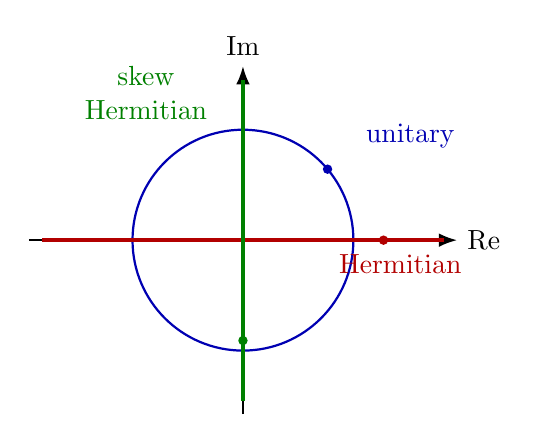
\begin{tikzpicture}[scale=0.85,>=Latex]
  \draw[->,thick] (-3.2,0) -- (3.2,0) node[right] {$\operatorname{Re}$};
  \draw[->,thick] (0,-2.6) -- (0,2.6) node[above] {$\operatorname{Im}$};
  \draw[blue!70!black,thick] (0,0) circle (1.65);
  \node[blue!70!black] at (2.5,1.55) {unitary};
  \node[red!70!black] at (2.35,-0.35) {Hermitian};
  \node[green!50!black,align=center] at (-1.45,2.2) {skew\\Hermitian};
  \draw[red!70!black,ultra thick] (-3,0) -- (3,0);
  \draw[green!50!black,ultra thick] (0,-2.4) -- (0,2.4);
  \fill[blue!70!black] ({1.65*cos(40)},{1.65*sin(40)}) circle (2pt);
  \fill[red!70!black] (2.1,0) circle (2pt);
  \fill[green!50!black] (0,-1.5) circle (2pt);
\end{tikzpicture}
\end{center}

\vfill

\begin{center}
\renewcommand{\arraystretch}{1.25}
\begin{tabular}{c|c}
$A^H=A$ & eigenvalues on real axis \\
$A^H=-A$ & eigenvalues on imaginary axis \\
$U^HU=I$ & eigenvalues on unit circle
\end{tabular}
\end{center}

\end{frame}


\begin{frame}{What Survives Over Real Numbers?}

The true machine is complex:

$$
A\text{ normal}
\quad\Longrightarrow\quad
\Omega^HA\Omega=\Lambda.
$$

\vfill\pause

For real applications, we ask:

\begin{center}
\x{When can the whole computation stay real?}
\end{center}

\vfill

That means:

\begin{itemize}
\item eigenvalues are real,
\item spectral projections have real entries,
\item diagonal cross-filling uses real vectors.
\end{itemize}

\end{frame}


\begin{frame}{Real Symmetric Matrices Stay Real}

If $A$ is real symmetric:

$$
A^T=A.
$$

\vfill\pause

Then $A^H=A$, so $A$ is Hermitian.

\vfill

Therefore all eigenvalues are real.

\vfill\pause

The Lagrange projection formula uses real roots:

$$
P_i=f_i(A),
\qquad
f_i(t)=\prod_{j\ne i}\frac{t-\lambda_j}{\lambda_i-\lambda_j}.
$$

\vfill

Since $A$ and the $\lambda_i$ are real, every $P_i$ is real.

\end{frame}


\begin{frame}{Real Orthogonal Diagonalization}

For a real symmetric matrix:

$$
P_i^H=P_i
\quad\text{becomes}\quad
P_i^T=P_i.
$$

\vfill\pause

Diagonal cross-filling uses only real numbers and produces real orthonormal eigenvectors.

\vfill

Stack them into a real matrix $Q$:

$$
Q^TQ=I,
\qquad
Q^TAQ=\Lambda.
$$

\vfill

\begin{block}{Real Specialization}
Real symmetric matrices admit real orthogonal diagonalization.
\end{block}

\end{frame}


\begin{frame}{Why Skew-Symmetric Real Matrices Leave $\mathbb{R}$}

If $A$ is real skew-symmetric:

$$
A^T=-A.
$$

\vfill\pause

Then $A^H=A^T=-A$, so $A$ is skew-Hermitian.

\vfill

Skew-Hermitian eigenvalues lie on the imaginary axis:

$$
\lambda\in i\mathbb{R}.
$$

\vfill\pause

So nonzero eigenvalues are usually not real.

\vfill

\x{This is why the complex world is necessary.}

\end{frame}


\begin{frame}{Real-World Summary}

\begin{center}
\renewcommand{\arraystretch}{1.5}
\scriptsize
\begin{tabular}{c|c|c}
\textbf{Real matrix type} & \textbf{Complex view} & \textbf{Real outcome}\\
\hline
$A^T=A$ & Hermitian & real orthogonal diagonalization\\
$A^T=-A$ & skew-Hermitian & imaginary eigenvalues\\
general real $A$ & may be non-normal & no orthogonal eigenspace guarantee
\end{tabular}
\end{center}

\vfill\pause

\x{Hermitian geometry is the real god:} real symmetric theory is its real shadow.

\end{frame}


\begin{frame}{Final Picture of Normal Matrices}

Normal matrices are the matrices whose spectral decomposition is orthogonal:

$$
\mathbb{C}^n
=E_{\lambda_1}\orthoplus\cdots\orthoplus E_{\lambda_k}.
$$

\vfill\pause

Special normal matrices add restrictions on eigenvalue locations:

\vfill

\begin{center}
\renewcommand{\arraystretch}{1.5}
\begin{tabular}{c|c}
Hermitian & real axis \\
Skew-Hermitian & imaginary axis \\
Unitary & unit circle
\end{tabular}
\end{center}

\vfill

\x{Key:} orthogonal eigenspaces first; eigenvalue geometry second.

\end{frame}

\end{document}
